\chapter{Reduced Requirement set} \label{ch:Reduced Requirement Set}
In this chapter the turtlebot and its requirements will be described.

\section{Turtlebot} %introduction
A Turtlebot is a prototype robot made for developers.\\
In this project the Turtlebot will be used as a prototype to test the different implementations. Due to the immense task of building a real rover in time for this project.\\
The Turtlebot consist of different parts, which will be described in this section.

\subsection{Base} %chassis
\begin{figure}[h]
    \centering
    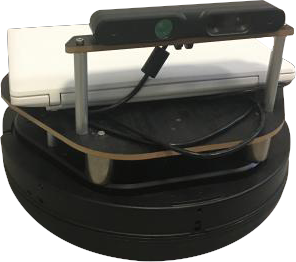
\includegraphics[width=.5\textwidth]{figures/turtlebot001.png}
    \caption{The turtlebot with new setup} 
    \label{fig:turtlebot} 
\end{figure}
The base is a Kobuki which purpose is to be used for prototyping and educational use. The base has two motors, which can move the robot at a velocity of 0.65 m/s. The motor is a 12V brushed DC motor which is controlled by a H-bridge that has been connected to the source.\\
The motors have an encoder on each wheel, which makes 11.5 ticks per millimetre of movement and 2578.33 ticks per full rotation.\\
The motors are protected from high current above 3 AMP. The maximum rotational velocity is 180 deg/s. The base has a gyro which works on the z-axis (110 deg/s calibrated from factory).\\
The base has three cliff sensors, these sensors are located in the center and to left and right. The base has a wheel drop sensor that detects if a wheel has dropped into a hole. The Base wheels can drive over obstacles with a height of 12 mm and the base can clear obstacles with a height of 15 mm. The base has two different batteries both on 14.8 VDC one has a capacity of 2200 mAh and the second one has a capacity of 4400 mAh.\\ 
The load capacity of the turtlebot is 5 kg on hard surface and on soft surfaces the load capacity is 4 kg \cite{Base}.

\subsection{Computer} 
The computer is an ASUS notebook, it has an Intel core i3-4010U CPU that has 2 cores and operate at 1.7MHz each \cite{CPU}. The notebook has 4 GB RAM and an integrated HD graphics card on its motherboard \cite{ASUS}.
The operating system is Ubuntu 16.04 LTS, a layer for the Linux distribution. For communication between the sensors and the Turtlebot, the computer uses USB 2.0.
\begin{figure}[h]
   \centering
    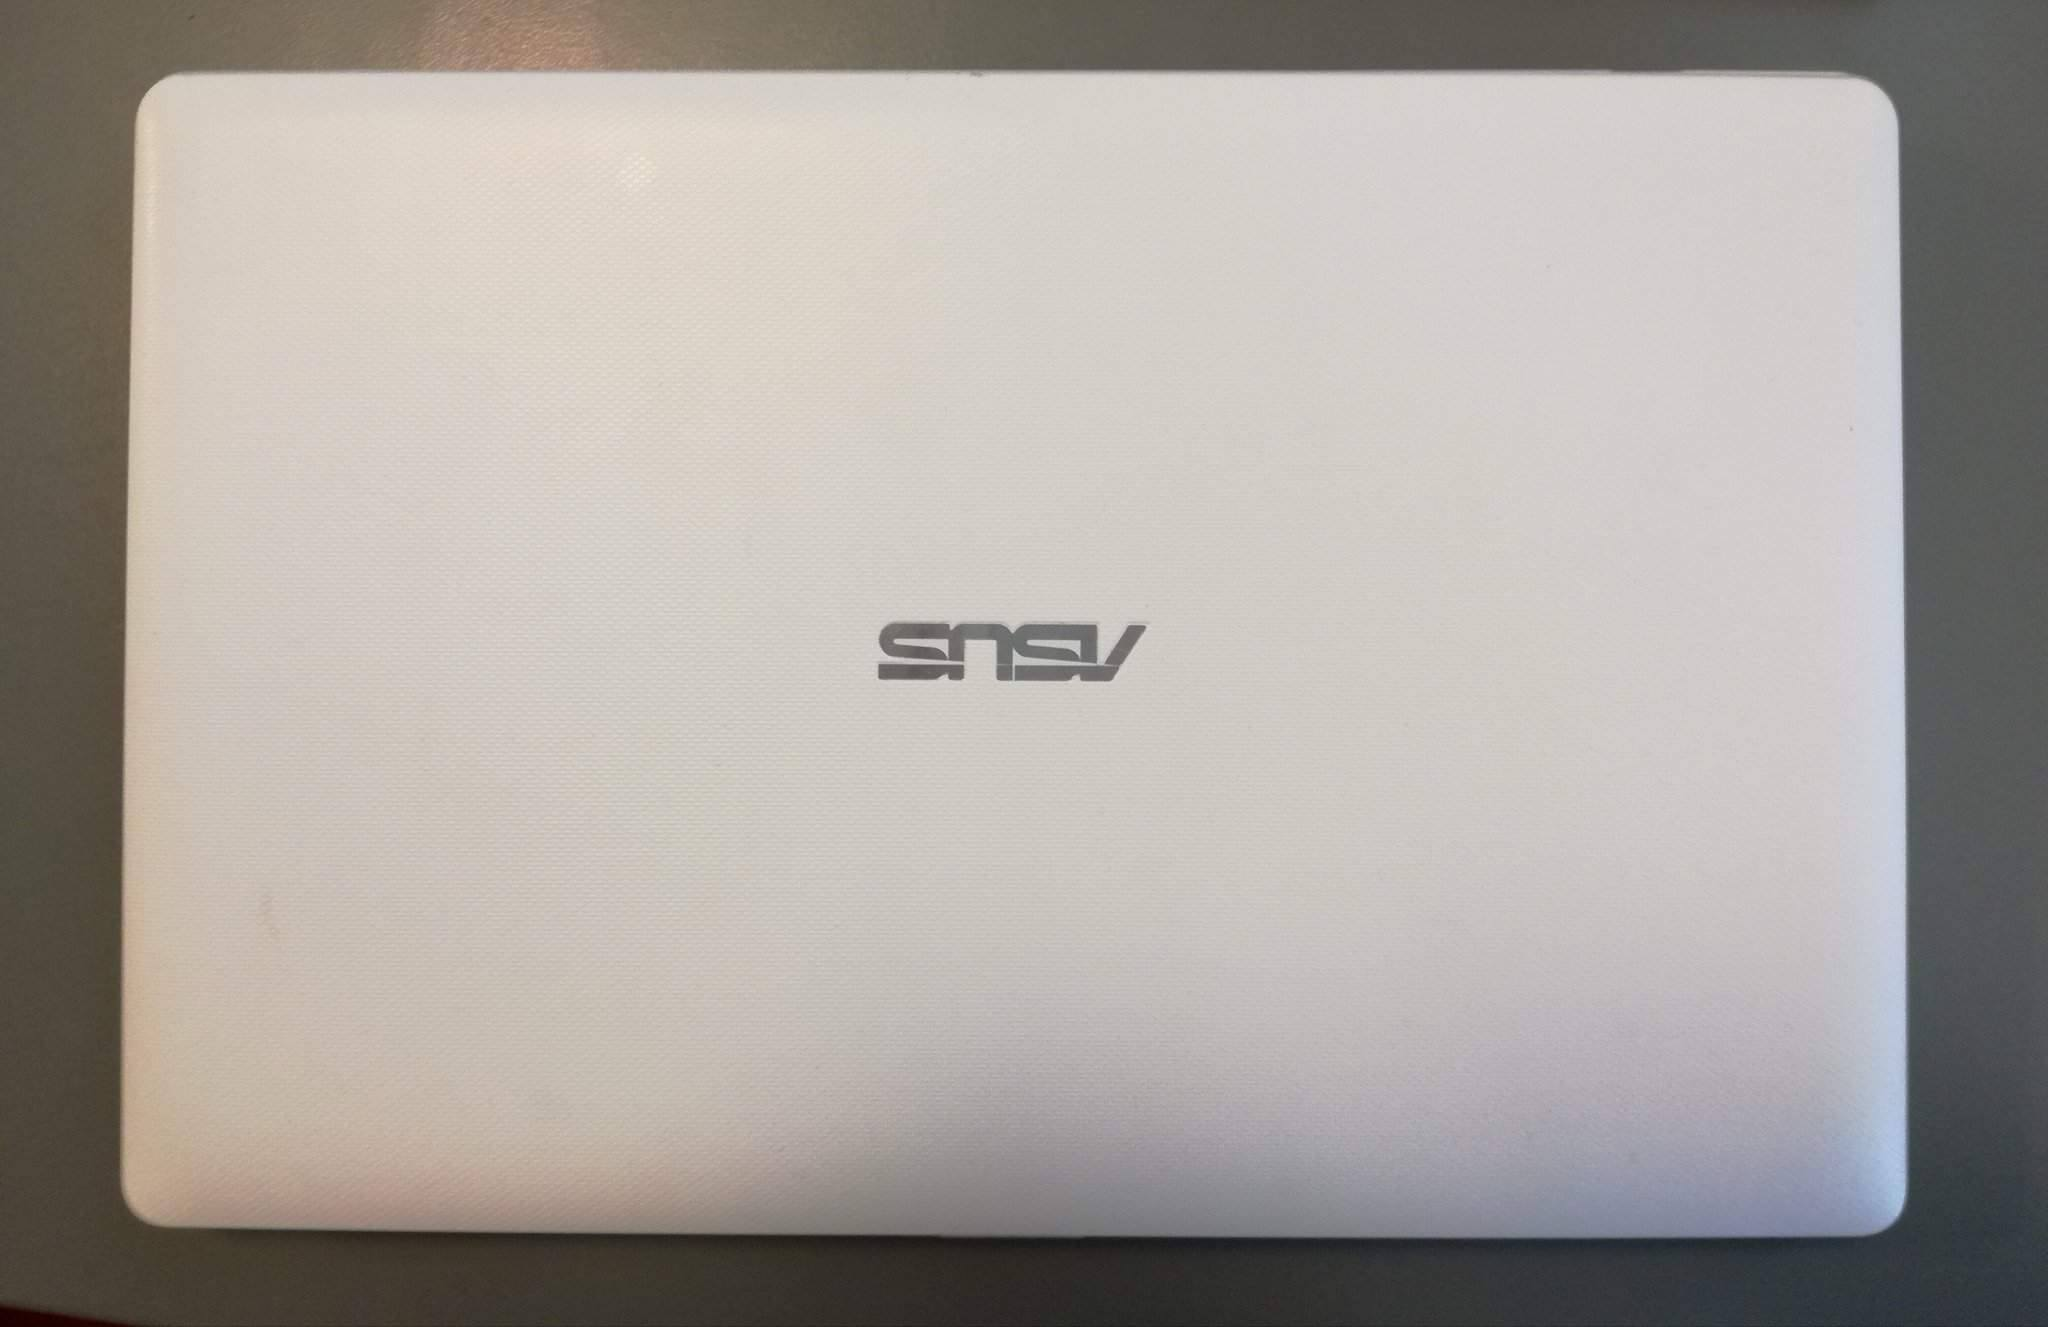
\includegraphics[width=.8\textwidth]{figures/ASUS.jpg}
    \caption{The computer used with the turtlebot}
    \label{fig:ASUS}
\end{figure}

\section{Requirements for the turtlebot}\label{ch:Requirements for the turtlebot}
It is required for the turtlebot to do the following:
\begin{itemize}
    \item The robot has to be able to drive with a distance of 8 m from the router without dropping the connection.
    \item It has to be able to move 5 m in 1 min.
    \item It has to be able to turn 360${^\circ}$ in less than a minute.
    \item The robot has to avoid obstacles with a height of more than 16 cm, with a distance of 20 cm away from the obstacles. 
    \item The robot needs to be able to detect obstacles, with a minimum height of 16 cm and a width of 3 cm, at a distance of up to 3.3 m.
    \item The robot needs to be able to detect ledges at distances of 2 m or more.
\end{itemize} 

